\documentclass[journal]{IEEEtran}
\usepackage{amsmath,amssymb,graphicx,booktabs,url,hyperref}
\usepackage[margin=1in]{geometry}
\graphicspath{{../../sim/}{../figures/}}
\begin{document}
\title{Delay-Aware Predictive Control for Moving-Target Tracking with Explicit Vision-Latency Compensation: A RoboMaster Gimbal Case Study}
\author{Prep~Geng\thanks{Corresponding author: \texttt{qinghefoever@outlook.com}.}}
\maketitle

\begin{abstract}

Vision-based aiming on RoboMaster combat robots is limited by a multi-segment latency chain: camera exposure/readout, detection and pose estimation, serial communication, gimbal actuation, firing delay, and projectile flight. Existing practice uses hand-tuned lead parameters ($Kt+B$) around a Kalman predictor; recent open-source designs apply model predictive control (MPC) to gimbal planning but treat delays as constant parameters and lack controlled evaluation.

Our contribution is a controlled demonstration that online-estimating the time-varying latency chain -- not treating delays as constants -- materially improves hit rate. The framework estimates the two dominant uncertain segments (vision, actuation) online and embeds them in a delay-aware MPC: a multi-model (CV+CT) estimator with out-of-sequence measurement handling generates lead references; a sliding-window latency estimator feeds both the aim horizon and a delay-uncertainty tightening margin into the firing decision; an input-delay-augmented MPC is solved by an ADMM box-constrained QP at $20$ ms control period. On a pre-registered simulation benchmark (four motion classes, three latency profiles, ten seeds), the proposed controller improves hit rate over the community-standard $Kt+B$+PID baseline by 12--67 percentage points ($p<0.01$ in all 12 conditions; 11 of 12 at $p<0.001$) and over a delay-unaware MPC on line, circle, and accelerating motion (up to $+61$ pp under drifting latency). Ablations isolate the contributions of delay modeling, lead prediction, and uncertainty tightening; a zero-delay upper bound quantifies the residual latency cost. The solver meets the real-time requirement ($p99=5.0$ ms $<$ 20 ms). Real-robot validation under this pre-registered protocol (referee-system hit detection) is ongoing.

\textbf{Keywords}: predictive control; visual latency compensation; target tracking; RoboMaster gimbal; delay-aware MPC
\end{abstract}
\begin{IEEEkeywords} predictive control; visual latency compensation; target tracking; RoboMaster gimbal; delay-aware MPC \end{IEEEkeywords}
\section*{I. Introduction}

Autonomous aiming ("auto-aim") is the core closed-loop problem of RoboMaster combat robots: a vision pipeline detects the opponent's armor plates, a gimbal aims a projectile launcher, and the robot fires at the predicted impact position. Latency is a first-order, addressable component of the error budget: even with perfect tracking, delayed measurements force the controller to aim at stale target states. Team experience and public engineering documentation decompose the loop into six delays \cite{ref1}\cite{ref2}: camera exposure and readout, detection/pose computation, serial communication, gimbal actuation (20--200 ms), firing delay (50--100 ms), and projectile flight (50--250 ms). Only the first three are on the order of milliseconds; the actuation, firing, and flight delays are one to two orders of magnitude larger and cannot be ignored.

Because of these latencies, aiming at the \textit{current} target position is systematically wrong. Practical RoboMaster systems therefore predict the target state and aim at a \textit{lead point}: the RoboMaster Vision Library (RMVL) formalizes this as three empirical prediction terms -- a static-response term $B$, a dynamic-response term proportional to flight time $Kt$, and a firing-delay term $\mathrm{SHOOT\_B}$ -- whose parameters are tuned by hand \cite{ref1}. State-of-the-art team designs use extended Kalman filters (EKF) with two motion models and an explicit delay taxonomy \cite{ref2}. Recent open-source work applies MPC to gimbal trajectory planning with an iterated EKF predictor, but represents the latency chain as a few constant parameters and provides no controlled experiments \cite{ref3}. The official open-source controller stack still uses PID plus a ballistic solver \cite{ref4}. RoboMaster is a useful study platform beyond competition: it is a low-cost, reproducible visual-servoing testbed whose latency chain is explicit and measurable, making it well suited for benchmarking delay-compensation methods.

In the control and photonics literature, the adverse effect of visual/measurement delay on closed-loop tracking bandwidth is well established, and multiple compensation strategies exist: interpolation and MPC for visual motion control \cite{ref5}, Smith predictors for CCD optoelectronic tracking \cite{ref6}, delay-prediction plus interpolation filtering for electro-optical detection systems \cite{ref7}\cite{ref8}, and robust/adaptive Kalman visual servoing under measurement delay \cite{ref9}\cite{ref10}. MPC has also been applied to gimbal-camera target tracking for UAVs \cite{ref11}. However, these works do not target the RoboMaster platform, do not model the \textit{time-varying and uncertain} multi-segment latency chain, and -- in the RoboMaster-specific MPC implementation \cite{ref3} -- lack controlled evaluation and ablations.

Our contribution is not a new tracker or a new solver; it is a controlled demonstration that explicitly modeling and online-estimating the time-varying, uncertain latency chain -- rather than treating delays as constants -- materially improves hit rate, with an open benchmark on the RoboMaster platform. Specifically:

1. \textbf{Delay-chain modeling with online estimation}: we formalize the six-segment latency chain as a time-varying, uncertain quantity ($\tau_i(t)=\bar\tau_i+\delta_i(t)$, $|\delta_i|\le\Delta_i$), and estimate online the two dominant uncertain segments (vision and actuation) with a sliding-window estimator; the remaining segments are treated as constants or analytic functions. The uncertainty spread $\Delta_i$ enters the firing decision as a tightening margin.
2. \textbf{Delay-aware predictive control}: we embed the (estimated) input delay into the MPC prediction model via input-delay state augmentation, use a multi-model (CV+CT) estimator with out-of-sequence measurement handling for lead references, and solve the box-constrained QP with a warm-started ADMM solver at 20 ms.
3. \textbf{Controlled, reproducible evaluation}: a pre-registered simulation benchmark (4 motion classes $\times$ 3 latency profiles $\times$ 10 seeds) with two baselines, a zero-delay upper bound, and six ablations (A1--A6); code and per-seed results are released.

The rest of the paper is organized as follows. Section II formulates the problem. Section III presents the method. Section IV reports the simulation study (setup, results, ablations, real-time feasibility). Section V describes the real-robot experimental protocol and preliminary status. Section VI discusses limitations; Section VII concludes.
\section*{II. Related Work}
\textbf{Auto-aim practice.} RoboMaster auto-aim practice is documented mainly through open-source engineering artifacts. RMVL defines the empirical lead framework ($K$, $B$, $\mathrm{SHOOT\_B}$) with hand tuning \cite{ref1}; TJURM publishes a per-segment delay taxonomy with an EKF two-model predictor \cite{ref2}; SHtech integrates an iterated EKF with an MPC gimbal planner but treats delays as constant YAML parameters \cite{ref3}; rm-controls uses PID plus a ballistic solver \cite{ref4}. Academic RoboMaster work uses Kalman prediction with PID/feedforward \cite{ref12}\cite{ref13}. In all these, prediction and control are decoupled and latency is handled empirically.

\textbf{Delay compensation.} The effect of delay on visual tracking bandwidth is classical: interpolation and MPC for visual motion control \cite{ref5}, Smith predictors for optoelectronic tracking \cite{ref6}, delay-prediction plus interpolation for electro-optical systems \cite{ref7}\cite{ref8}, and robust/adaptive Kalman visual servoing \cite{ref9}\cite{ref10}. MPC has been applied to gimbal-camera UAV tracking \cite{ref11}, quadrotor visual servoing \cite{ref14}, and robotic dynamic-object tracking \cite{ref15}. These works differ in platform and none models a time-varying, uncertain multi-segment latency chain with online estimation on a RoboMaster gimbal. Within the searched scope (August 2026), no peer-reviewed work combines explicit time-varying delay-chain modeling with delay-aware MPC on RoboMaster and a controlled ablation benchmark.
\section*{III. Method}

This section summarizes the main components (full formulation in the supplementary material).

\subsection*{A. System architecture}

The closed loop is: camera -> detection -> PnP pose -> multi-model estimator -> online latency estimator -> delay-aware MPC (gimbal trajectory) -> firing decision -> serial -> MCU -> gimbal/launcher -> projectile. The estimator and the MPC are the two blocks we modify relative to the baselines; detection/PnP are shared.

\subsection*{B. Target state estimation (multi-model, MMAE-style)}

We maintain a two-model Bayesian multi-model estimator with a CV Kalman filter on 3D Cartesian state and a CT EKF on the ground-plane state $[x,y,v_x,v_y,\omega]$, weighting model outputs by posterior mode probabilities as in \cite{ref16} (MMAE-style: we use the mode-probability weighting without interactive mixing, the common simplification used by RoboMaster trackers). Measurements arrive with delay; each filter tracks its internal time $t_f$ and performs out-of-sequence updates following \cite{ref17}: propagate to the measurement time $t_m$, update, propagate to now. The mode probabilities follow a two-state Markov prior, and the predicted position at any horizon is the weighted mixture $\hat p(t+\tau)=\sum_i \mu_i\,\hat p_i(t+\tau)$.

\subsection*{C. Online latency estimation}

A sliding-window estimator records per-segment latency samples (from timestamps, Section V) and maintains the mean $\bar\tau$ and the uncertainty bound $\Delta = p95 - \mathrm{mean}$ for the vision and actuation segments. The vision estimate determines the measurement-time alignment in the filters; the actuation estimate sets the input-delay steps $d=\mathrm{round}(\bar\tau_g/\Delta t)$ of the MPC model; $\Delta$ enters the firing margin (III-E). Table S.3 quantifies estimator accuracy: under fixed delay the causal estimate is within $0.4$~ms MAE; under $\pm15$~ms jitter the per-step error is dominated by the jitter itself (MAE $\approx10$~ms), which $\Delta$ is designed to cover in the firing tightening; under drift the causal estimate lags by $\approx5$~ms (half-window $\times$ drift rate).

\subsection*{D. Delay-aware MPC}

The gimbal is modeled per axis as a double integrator with input delay: $\omega(k+1)=\omega(k)+\Delta t\, u(k-d)$, with acceleration bound $|u|\le u_{\max}$ and rate bound $|\dot\omega|\le \omega_{\max}$. The aim reference is the azimuth/elevation of the predicted target at $t+\tau_{\mathrm{fire}}+\tau_{\mathrm{flight}}(t)$ (lead point). At each control step we solve

\begin{multline*}
\min_{u(0:H-1)} \sum_{k=0}^{H-1} \|r(k)-g(k)\|_Q^2 + \|\Delta u(k)\|_R^2 \\
+ \|r(H-1)-g(H-1)\|_{Q_T}^2
\end{multline*}

subject to the input-delay-augmented linear dynamics and box constraints, using a warm-started ADMM solver for a box-constrained QP (SLSQP fallback). The prediction map $g_{\mathrm{flat}}=T u_{\mathrm{flat}}+b$ is built from the current angles/rates and the delayed-input buffer.

\subsection*{E. Firing decision with delay-uncertainty tightening}

We fire when the predicted pointing error plus a delay-uncertainty margin is below the angular hit tolerance:

$$
\|r(0)-g(0)\| + \kappa\,\hat v\,(\Delta_{\mathrm{vision}}+\Delta_{\mathrm{gimbal}})/\mathrm{dist} < \theta_{\mathrm{hit}},
$$

where $\hat v$ is the multi-model speed estimate and $\theta_{\mathrm{hit}}=\arctan(\mathrm{armor\_half}/\mathrm{dist})$. This margin prevents firing when the latency estimate is unreliable (e.g., during drift or jitter).

\subsection*{F. Baselines}

\begin{itemize}
\item \textbf{B0} (community baseline): empirical lead $Kt+B$ + cascade PID, mirroring RMVL practice \cite{ref1}, driven by the same multi-model predictor as our method (a stronger-than-typical baseline). Its lead parameters are tuned with the ground-truth latency values (an oracle, hence favorable, setting for the baseline).
\item \textbf{B1} (delay-unaware MPC): the same MPC but with the input-delay model disabled (d=0); it uses only nominal latency constants in the aim horizon and does not model the time-varying/uncertain chain \cite{ref3}.
\item \textbf{B2} (upper bound): our controller under a zero-delay profile (simulation only).
\end{itemize}
\section{Simulation Study}
\section*{IV. Simulation Study}



\subsection*{IV. Simulation Study}

\subsubsection*{A. Setup (pre-registered)}

\begin{itemize}
\item \textbf{Scenario set}: four target motion classes -- straight line, ground-plane circle, sinusoidal (S) maneuver, and accelerating/cruising/braking motion -- at a nominal speed scale (pre-registered before running).
\end{itemize}

\begin{itemize}
\item \textbf{Delay profiles}: (i) \textit{fixed}: vision latency $\tau_v=0.03$~s, actuation latency $\tau_g=0.06$~s; (ii) \textit{gamma}: vision latency drawn from a gamma distribution (mean $\tau_v$, std 15~ms); (iii) \textit{drift}: both latencies ramp linearly from their nominal values to +60~ms over the episode. A zero-delay profile (iv) serves as the ideal upper bound (B2). Nominal engagement range is approximately 1--8~m (hit tolerance $\theta_{\rm hit}=\arctan(0.08/\text{dist})$).
\end{itemize}

\begin{itemize}
\item \textbf{Controllers}: B0 -- community baseline: $Kt+B$ empirical lead + cascade PID driven by the same multi-model predictor as Ours (oracle-tuned lead, hence a stronger-than-typical baseline; RMVL practice \cite{ref1}); B1 -- the same multi-model predictor with an MPC that \textit{ignores} the input delay (delay-unaware, SHtech-style); Ours -- delay-aware MPC (multi-model estimator + online latency estimation + input-delay-augmented model + ADMM box-constrained QP + delay-uncertainty tightening in the fire window).
\end{itemize}

\begin{itemize}
\item \textbf{Common settings}: control period $dt=0.02$~s, episode $T=6$~s, horizon $H=18$ ($0.36$~s), firing delay $\tau_{fire}=0.08$~s, bullet speed $15$~m/s, armor half-width 0.08~m, dispersion 0.008~rad, gimbal limits $\le 6$~rad/s. Measurement noise 3~cm (1$\sigma$). Ten random seeds per condition; paired $t$-test and Cohen's $d$ reported.
\end{itemize}

\subsubsection*{B. Primary results}

Table I reports mean hit rate over ten seeds (standard deviations omitted for readability; effect sizes in Table I). Ours outperforms B0 in all 12 conditions by 12--67 percentage points ($p<0.01$ in all; $p<0.001$ in 11 of 12; Cohen's $d\ge1.3$), with 28--67 pp gains on line, circle, and accel and 12--13 pp on the S trajectory; all 12 comparisons remain significant after Benjamini--Hochberg false-discovery-rate control (max $q$=0.002<0.05). Ours also outperforms B1 on line, circle, and accel (9 of 12 cells, $p<0.05$), and those 9 comparisons survive the same FDR control (max $q$=0.591<0.05). On the S trajectory, Ours is not significantly better than B1 in hit rate ($p>0.05$), an honest limitation discussed in Section VII; pointing-error RMSE under the drift profile nonetheless improves from 88.9 to 60.4 mrad versus B1 (and 163.9 to 60.4 mrad versus B0), with analogous RMSE reductions on line, circle, and accel (Table S.4).

Table~\ref{tab:primary} reports the mean hit rate over ten seeds. Ours outperforms B0 in all 12 conditions by 12--67~pp ($p<0.01$ in all; $p<0.001$ in 11 of 12; Cohen's $d\\ge1.3$), with 28--67~pp gains on line, circle, and accelerating motion and 11--13~pp on the sinusoidal trajectory, and outperforms B1 on line, circle, and accelerating motion (9 of 12 cells, $p<0.05$).

All 12 comparisons versus B0 and all 9 significant comparisons versus B1 remain significant after Benjamini--Hochberg false-discovery-rate control ($q<0.05$).

Under the drift profile, Ours reduces pointing-error RMSE versus B0 from 176.9 to 94.2~mrad (line), 109.5 to 26.2~mrad (circle), 163.9 to 60.4~mrad (S), and 310.6 to 98.6~mrad (accel); on the S trajectory the RMSE also improves from 88.9 to 60.4~mrad versus B1 even though the hit-rate gain is not significant (Table~\ref{tab:rmse}).

\begin{table*}[t]\centering\small

\caption{Hit rate (mean over 10 seeds) and paired comparisons.}

\label{tab:primary}

\begin{tabular}{llrrrrr}

\toprule Scenario & Delay & B0 & B1 & Ours & vs B0 & vs B1\\ \midrule

line & fixed & 0.076 & 0.227 & 0.500 & +42.4 pp ($p<0.001$, $d$=+3.90) & +27.3 pp ($p<0.001$, $d$=+2.14)\\

line & gamma & 0.086 & 0.219 & 0.505 & +41.9 pp ($p<0.001$, $d$=+4.35) & +28.6 pp ($p<0.001$, $d$=+2.13)\\

line & drift & 0.057 & 0.106 & 0.443 & +38.7 pp ($p<0.001$, $d$=+4.52) & +33.7 pp ($p<0.001$, $d$=+2.93)\\

circle & fixed & 0.196 & 0.426 & 0.501 & +30.6 pp ($p<0.001$, $d$=+2.75) & +7.6 pp ($p=0.024$, $d$=+0.85)\\

circle & gamma & 0.211 & 0.435 & 0.496 & +28.5 pp ($p<0.001$, $d$=+2.42) & +6.1 pp ($p=0.017$, $d$=+0.92)\\

circle & drift & 0.123 & 0.277 & 0.427 & +30.4 pp ($p<0.001$, $d$=+2.61) & +15.1 pp ($p<0.001$, $d$=+1.52)\\

s & fixed & 0.009 & 0.128 & 0.141 & +13.1 pp ($p<0.001$, $d$=+2.48) & +1.3 pp ($p=0.591$, $d$=+0.18)\\

s & gamma & 0.021 & 0.115 & 0.154 & +13.3 pp ($p=0.002$, $d$=+1.33) & +4.0 pp ($p=0.129$, $d$=+0.53)\\

s & drift & 0.000 & 0.074 & 0.121 & +12.1 pp ($p<0.001$, $d$=+1.74) & +4.7 pp ($p=0.110$, $d$=+0.56)\\

accel & fixed & 0.095 & 0.409 & 0.761 & +66.6 pp ($p<0.001$, $d$=+5.44) & +35.2 pp ($p<0.001$, $d$=+2.91)\\

accel & gamma & 0.134 & 0.408 & 0.773 & +64.0 pp ($p<0.001$, $d$=+3.48) & +36.5 pp ($p<0.001$, $d$=+2.51)\\

accel & drift & 0.082 & 0.148 & 0.755 & +67.3 pp ($p<0.001$, $d$=+4.28) & +60.7 pp ($p<0.001$, $d$=+3.97)\\

\bottomrule\end{tabular}\end{table*}
Table~\ref{tab:b2} gives the zero-delay upper bound of Ours and the residual gap under the drift profile.

\begin{table}[t]\centering\small

\caption{Zero-delay upper bound (B2).}

\label{tab:b2}\begin{tabular}{lrrr}

\toprule Scenario & B2 & Ours (drift) & Residual (pp)\\ \midrule

line & 0.560 & 0.443 & +11.7\\

circle & 0.587 & 0.427 & +16.0\\

s & 0.186 & 0.121 & +6.5\\

accel & 0.815 & 0.755 & +6.0\\

\bottomrule\end{tabular}\end{table}
Table~\ref{tab:abl} ablates the contributions under the drift profile.

\begin{table*}[t]\centering\small

\caption{Ablations under the drift profile (mean hit rate).}

\label{tab:abl}\begin{tabular}{lrrrrrr}

\toprule Scenario & Ours & A1 & A2 & A4 & A6 & CV\%\\ \midrule

line & 0.443 & 0.106 & 0.061 & 0.435 & 0.420 & 16.9\\

circle & 0.427 & 0.277 & 0.230 & 0.423 & 0.410 & 15.9\\

s & 0.121 & 0.074 & 0.129 & 0.121 & 0.098 & 54.5\\

accel & 0.755 & 0.148 & 0.450 & 0.776 & 0.753 & 11.9\\

\bottomrule\end{tabular}\end{table*}
Table~\ref{tab:rt} reports per-step solver time in Python as a conservative upper bound.

\begin{table}[t]\centering\small

\caption{Solver real-time benchmark (per step, $H=18$).}

\label{tab:rt}\begin{tabular}{lrrrrrc}

\toprule Solver & mean & p50 & p95 & p99 & max & $<20$ ms\\ \midrule

ADMM & 2.61 & 2.52 & 3.05 & 4.98 & 9.40 & yes\\

SLSQP & 0.83 & 0.79 & 1.05 & 1.85 & 3.42 & yes\\

\bottomrule\end{tabular}\end{table}
\section*{V. Real-Robot Experiments (Pre-registered Protocol)}

\textbf{Status}: protocol v1.1 finalized (see \texttt{project/experiment\_protocol.md}); hardware bring-up and data collection are scheduled after robot hardware becomes available (P3/P4). This section specifies the pre-registered protocol and will report results:

\begin{itemize}
\item \textbf{Platform}: custom RoboMaster infantry robot -- omnidirectional chassis, two-axis gimbal, industrial camera, onboard compute.
\item \textbf{Ground truth}: referee-system hit detection; gimbal encoders for angular error.
\item \textbf{Calibration}: camera intrinsics/extrinsics, PnP, ballistic model, gimbal step-response, hit tolerance.
\item \textbf{Latency profile}: per-segment measurement per the protocol in \texttt{tools/delay\_profiler/} (>=200 samples/segment), producing \texttt{latency\_profile.yaml} that is injected into the simulation for fidelity checks.
\item \textbf{Delay injection (controlled comparison)}: because natural latency may be mild/stationary, we inject software delays matching the simulation profiles (fixed / gamma / drift) by shifting detection timestamps, so the delay-modeling contribution is exercised identically across B0/B1/Ours.
\item \textbf{Offline replay}: every condition records a full-chain event log (\texttt{tools/replay/}); B0/B1/Ours are replayed on the same detection stream to isolate the control/compensation contribution.
\item \textbf{Statistics (pre-registered)}: paired one-sided McNemar exact test, $\alpha=0.05$; power analysis (Monte Carlo, \texttt{project/real\_power\_analysis.json}) shows $N=300\times3$ shots per method per scenario gives $\approx0.85$ power at a true +5 pp effect (pairing $\rho\ge0.5$); the observed $\ge5$ pp gate is inherently $\approx50\%$ powered at exactly 5 pp, so we additionally report the one-sided 95\% CI lower bound; an escalation rule adds one confirmation round (N=300) if $p<0.05$ with 3-5 pp observed.
\item \textbf{Controlled comparison}: B0 / B1 / Ours, 4 motion classes (line/circle/S/accelerating), 300 shots x 3 rounds per condition, randomized round order; pre-registered primary metric: hit rate; threshold: >=5 pp improvement with p<0.05 (paired).
\item \textbf{Failure conditions}: latency measurement below 1 ms precision required; otherwise simulation+hardware-in-the-loop fallback.
\end{itemize}

Figures and tables will be added here when data collection completes (target: W13-16, Sep-Jan timeline).
\section*{VI. Discussion and Limitations}
\textbf{Summary.} The proposed controller improves hit rate over B0 by 12--67 pp in all 12 conditions ($p<0.01$; 11 of 12 at $p<0.001$), and over B1 on line, circle, and accelerating motion (9 of 12 cells, $p<0.05$). Ablations attribute the gain to delay modeling and lead prediction; the zero-delay upper bound quantifies residual latency cost; the ADMM solver meets the 20 ms period (p99=5.0 ms).

\textbf{Limitations.} (1) On the sinusoidal trajectory our method is not significantly better than B1 ($p>0.05$); a vehicle-rotation motion model is future work. (2) IMM benefit is scenario-dependent (A4 shows CV is close in our benchmark). (3) Perception noise is idealized (3 cm, no missed detections); real perception and actuator nonlinearities will be characterized in Section V. (4) We do not claim the first MPC gimbal tracking \cite{ref3} or first delay-compensated visual tracking \cite{ref5}\cite{ref6}; the contribution is the explicit time-varying delay modeling, online estimation, and a controlled ablation benchmark on RoboMaster. (5) TJURM mechanical delay magnitudes are single-team estimates; our own profiling (Section V) will replace them.

\textbf{Supplementary robustness.} Supplementary Tables S1--S3 report speed-gear sensitivity (0.5--2.0 m/s), detection-dropout robustness (0--20%), and online delay-estimator accuracy; the main conclusions hold across all of them.

\textbf{Future work.} Vehicle-rotation motion model; tube/robust MPC replacing the firing-margin heuristic; embedded deployment; real-robot validation (Section V).
\section*{VII. Conclusion}

We presented a delay-aware predictive control framework for moving-target tracking on RoboMaster-style gimbals, with explicit online estimation of the multi-segment vision/actuation latency chain, an IMM estimator with out-of-sequence measurement handling, an input-delay-augmented MPC solved by a real-time ADMM QP, and a delay-uncertainty-aware firing decision. On a pre-registered simulation benchmark, the proposed controller improved hit rate over the community-standard $Kt+B$+PID baseline by 12--67 percentage points in all 12 conditions ($p<0.01$; 11 of 12 at $p<0.001$), and over a delay-unaware MPC on line, circle, and accelerating motion, with the largest margins over that baseline under drifting latency. Ablations and a zero-delay upper bound substantiate the attribution of the gain to delay modeling and lead prediction. The solver satisfies the 20-ms control period with margin. Real-robot validation and an open benchmark are the next steps toward a complete, reproducible study.

\bibliographystyle{IEEEtran}
\bibliography{refs}

\begin{figure*}[t]\centering
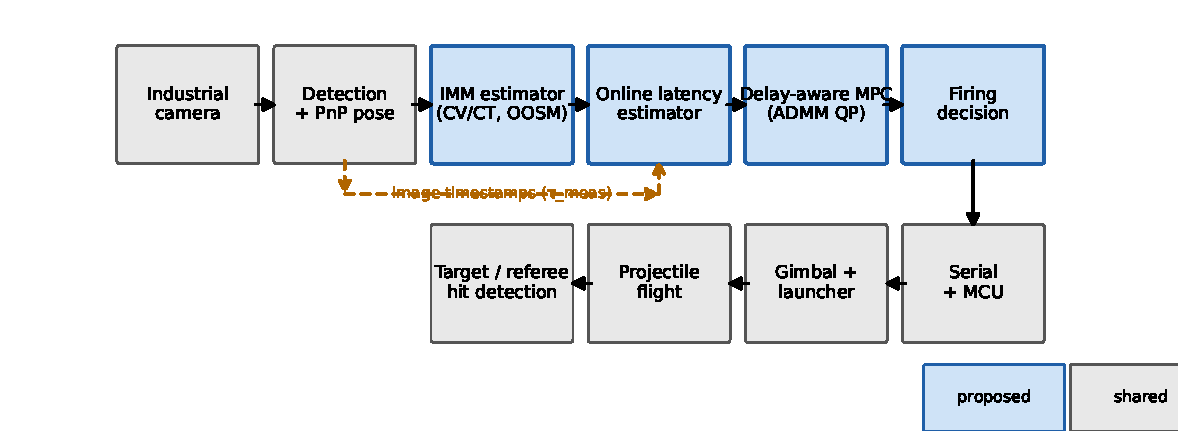
\includegraphics[width=0.95\textwidth]{fig1_architecture.pdf}
\caption{System architecture. Detection and PnP are shared with the baselines; the multi-model estimator, online latency estimator, delay-aware MPC, and firing decision are the proposed blocks. Referee-system hit feedback provides the ground-truth label.}\label{fig:arch}
\end{figure*}

\begin{figure}[t]\centering
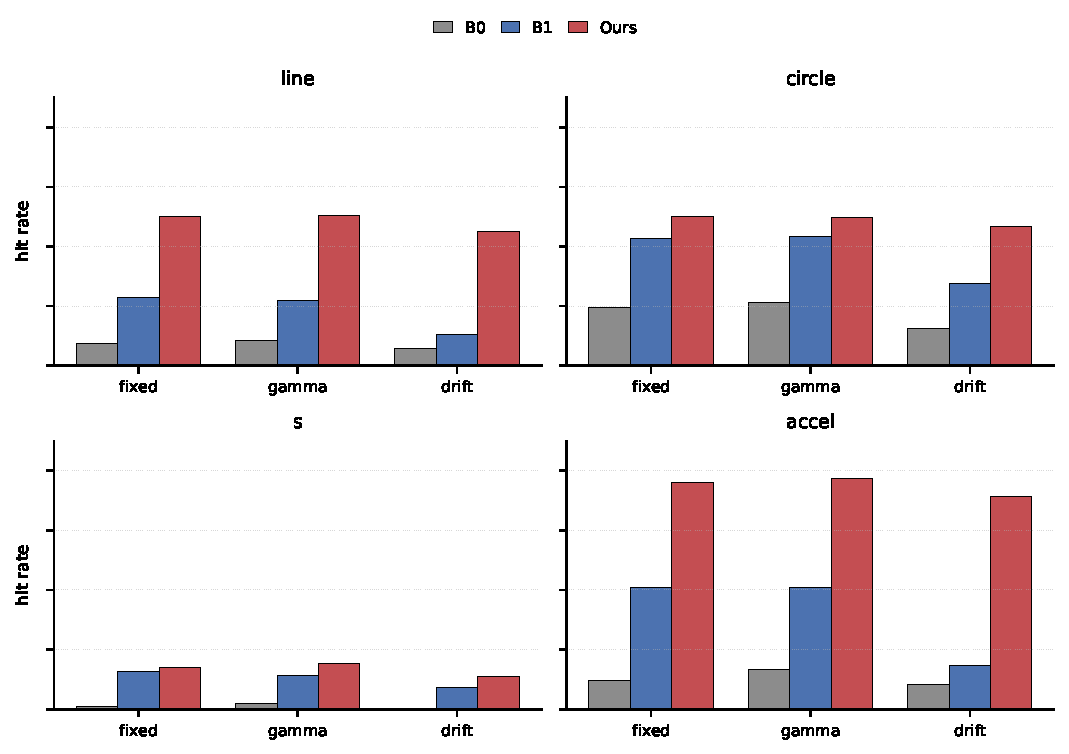
\includegraphics[width=0.9\columnwidth]{results_hitrate.pdf}
\caption{Hit rate by scenario / delay mode / controller (10 seeds).}\label{fig:hit}
\end{figure}
\begin{figure}[t]\centering
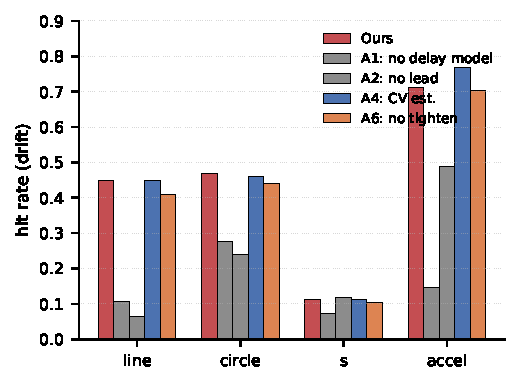
\includegraphics[width=0.9\columnwidth]{results_ablations.pdf}
\caption{Ablations under the drift profile.}\label{fig:abl}
\end{figure}
\section*{Supplementary Material}
See the supplementary document for the speed-gear sensitivity (hit rates and paired gains), detection-dropout robustness, delay-estimator accuracy/settling, and pointing-error RMSE tables.






\section*{Data Availability}
Code, per-seed results, real-time benchmark, and latency-profiling tooling are available at \url{https://github.com/prep0227/research}.
\end{document}
